\newpage
%\section{Background Theory}
\chapter{Background Theory}
\label{sec:theory}

\section{Hyperspectral imaging}
\subsection{AVIRIS}
The Airborne Visible Infrared Imaging Spectrometer (AVIRIS) is a hyperspectral imager launched by NASA. Its main objective is to "identify, measure and monitor constituents of the Earth's surface and atmosphere" \cite{aviris}. 
\subsubsection{Cuprite scene}
Data from the Cuprite mining district \cite{Cuprite_data} captured by the AVIRIS imager is often used as a benchmark scene for different image processing algorithms, including anomaly detection algorithms. Scene 02 from the Cuprite mining can be seen in Figure \ref{fig:cuprite_mining_scene}. 12 different mineral with their respective spectral signature are extracted from the scene \cite{aviris_minerals}. The spectral signatures of the different minerals can be seen in Figure \ref{fig:minerals_Cuprite}. 

\begin{figure}[H]
\hbox{\hspace*{-1cm}                                              
   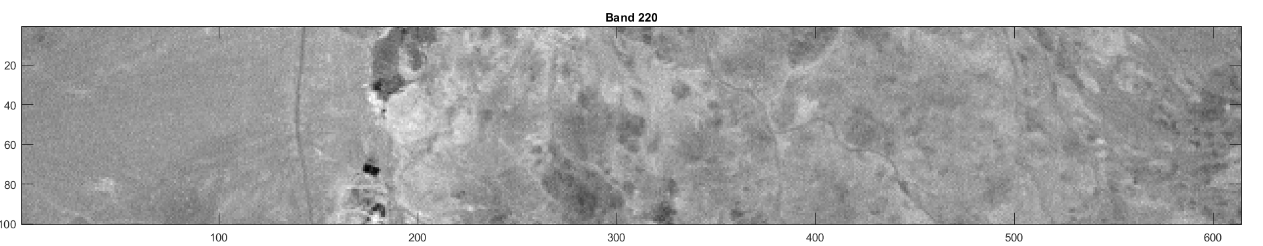
\includegraphics[scale=0.55]{images/AD_testing/original_band_220_22_1.png}}
  \caption{ Band 220 from the Cuprite scene 02 \cite{Cuprite_data}. } 
  \label{fig:cuprite_mining_scene}
\end{figure}

\begin{figure}[H]
\hbox{\hspace*{-1.0cm}                                              

   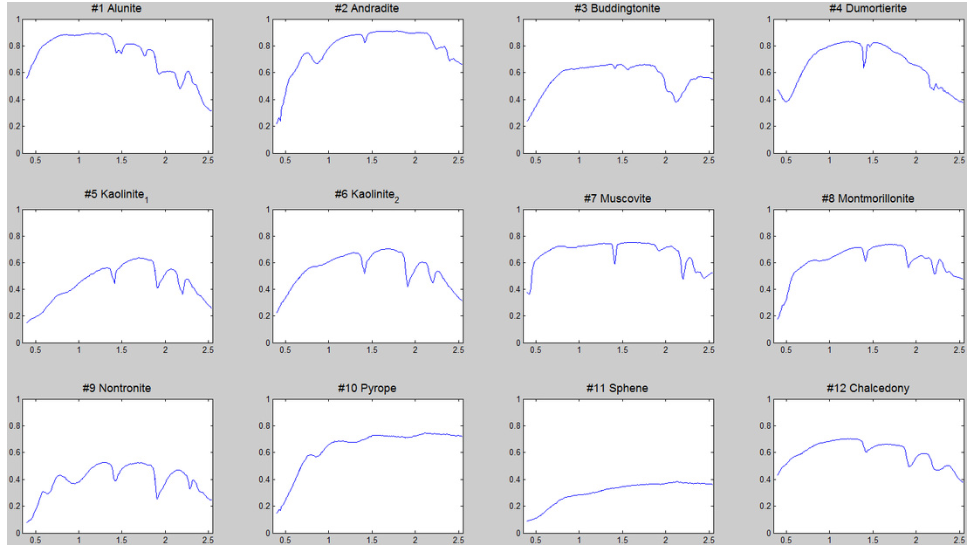
\includegraphics[scale=0.7]{images/AD_testing/endmembers_Cuprite.PNG}}
  \caption{ Spectral signatures of minerals from the Cuprite mining district \cite{aviris_minerals}. } 
  \label{fig:minerals_Cuprite}
\end{figure}


\subsection{NTNU Smallsat Project}

The hyperspectral imager used in the NTNU SmallSat project has 100 usable bands, $N_{bands}$, with a sensor resolution of 2048 x 1088 pixels. The number of effective pixels, $N_{pixels}$, is 578. This is the number of effective pixels per row in the image. The number of pixel rows, $N_{rows}$, is 1088. The hyperspectral image cube can be seen in Figure \ref{fig:HSI_image_cube}. Figure \ref{fig:HSI_functionality} displays the functionality of the hyperspectral imager. The imager captures data one pixel at the time, in a row-wise fashion \cite{SmallSat_project_description}.

\textbf{\begin{figure}[H]
\centering
   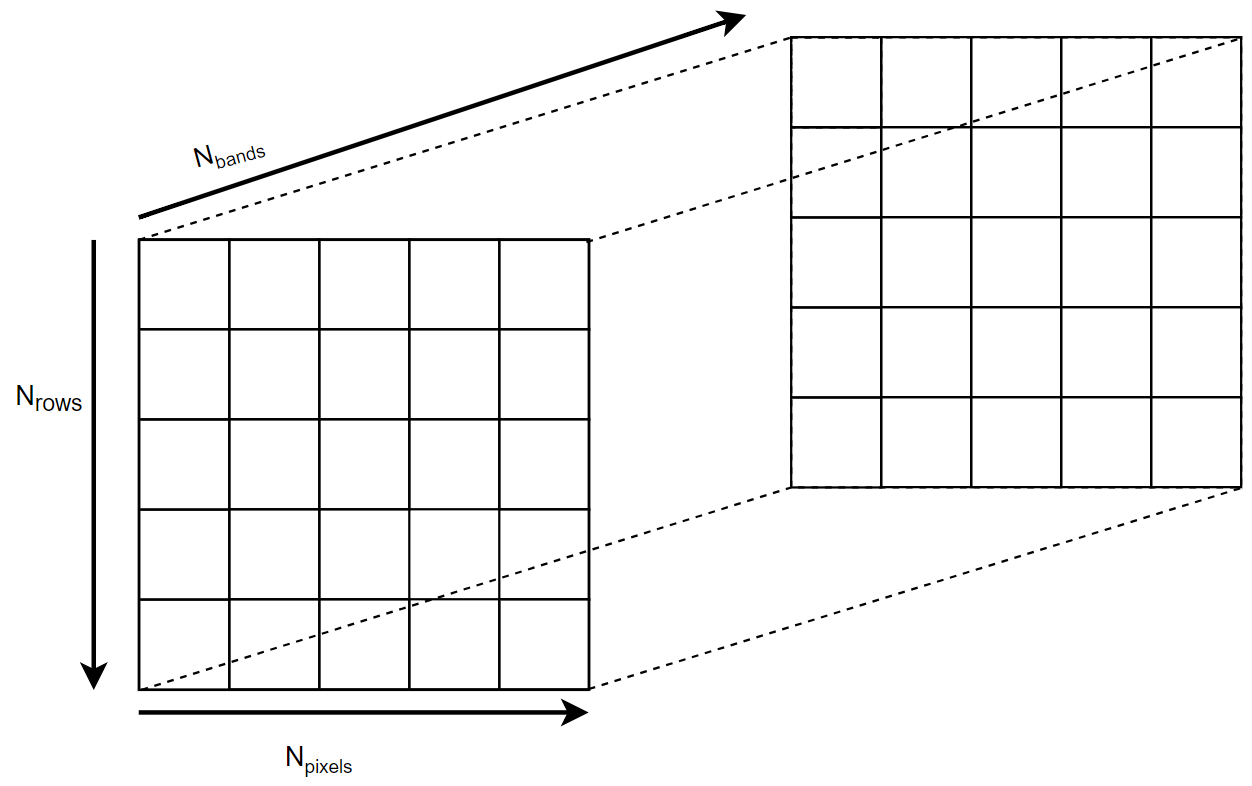
\includegraphics[scale=0.4]{images/hsi_image_cube.PNG}
  \caption{ Hyperspectral image cube.} 
  \label{fig:HSI_image_cube}
\end{figure}}

\begin{figure}[H]
\centering
   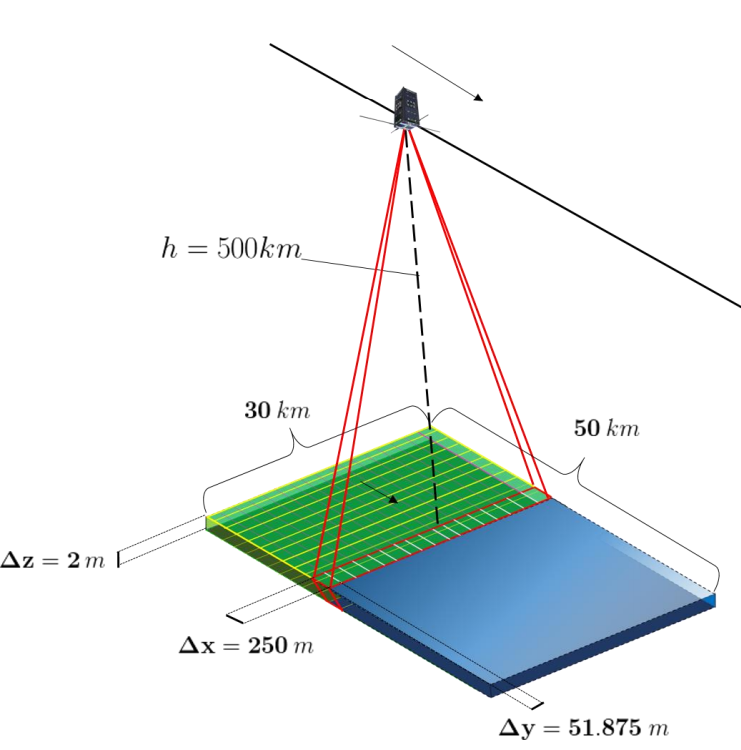
\includegraphics[scale=0.36]{images/hyperspectral_imager.PNG}
  \caption{ Push-broom hyperspectral imager mode of operation \cite{SmallSat_project_description}.  } 
  \label{fig:HSI_functionality}
\end{figure}

\section{NTNU Smallsat Project Hardware platform}
The NTNU SmallSat project onboard processing system is a Zynq-7000 series System-on-Chip (SoC). The SoC can be divided into two parts; the programmable system and the programmable logic. This is shown in Figure \ref{fig:zynq_7000}. The programmable system consists of a dual core ARM Cortex A9. The programmable logic main processing unit is a Artix-7 or Kintex-7 Series FPGA, depending upon the version of the Zynq-7000 series.


\begin{figure}[H]
\centering
   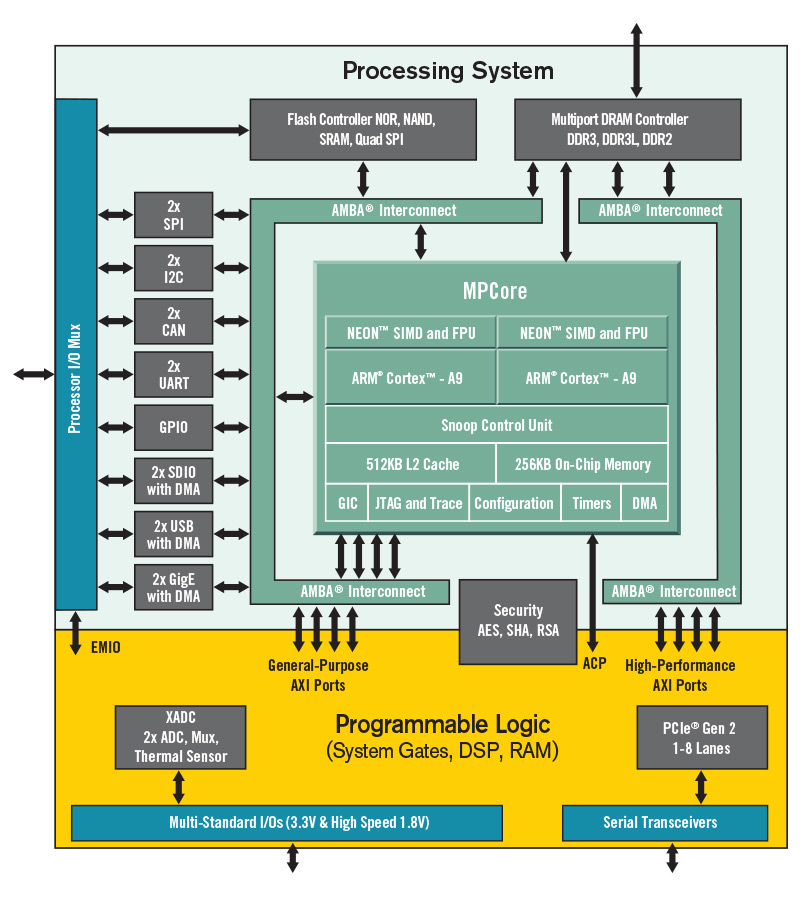
\includegraphics[scale=0.3]{images/zynq-mp-core-dual.png}
  \caption{ Zynq-7000 architecture \cite{cite:zynq_7000}. } 
  \label{fig:zynq_7000}
\end{figure}
 In NTNU SmallSat Project, an initial prototype will be developed on a Zynq Zedboard Evaluation and Development kit, featuring a Zynq-Z7020, which contains an Artix-7 device. Later stage prototypes will feature Zynq-Z7030 or Z-7035. These contains Kintex-7 devices. 

\\
The anomaly detection result will be transmitted from the satellite to a ground base station. The data budget for packet transmissions are as in page 23 in \cite{SmallSat_project_description}. The size of the AD result must be as small as possible to limit the anomaly detection data packet usage.  

\subsection{AXI-Stream}
AXI-Stream is a slimmed-down protocol for transfers, without any concept of addresses, where data is moved from one point to another. It is based on the read and write channels in the AXI protoicol. As for AXI buses, handshaking signals (\textbf{TREADY} and \textbf{TVALID}) are used when transferring data. A handshake of data is called a \textit{beat} according to the AXI and AXI-Lite specifications. \\

The NTNU SmallSat utilizes AXI-Lite as the communication protocol between Intellectual Properties (IP). The operating frequency of the AXI-Lite protocol in the NTNU SmallSat project is 100 MHz. 


\section{Anomaly detection}
\label{sec:anomaly_detectors_theory}
The process of detecting anomalies in a hyperspectral image is called anomaly detection. For a spectral vector to be considered as an anomaly, it has to be significantly different to its neighboring background. Four issues arising in anomaly detection is \cite{chang2006characterization}:
\\
 
\begin{itemize}
  \item Q1: How large for a target to be considered as an anomaly?
  \item Q2: How does an anomaly respond to its neighbouring pixels?
  \item Q3: How sensitive is anomaly detection to noise?
  \item Q4: How are different anomalies to be detected and classified?
\end{itemize}

The above-mentioned issues are important for the choice of anomaly detection algorithm, and will be further discussed in this chapter.
\\
Algorithms used for anomaly detection outputs a scalar for each pixel in an image indicating the relative probability that the spectral pixel vector is an anomaly. A higher output indicates a higher probability for the pixel vector being an anomaly.
%\subsection{Background compression}
% See book

%\subsection{Causality}

\subsection{Reed-Xiaoli algorithm}
\label{sec:RX_theory}
The Reed-Xiaoli (RX) algorithm \cite{reed1990adaptive} is one of the most widely used algorithms for anomaly detection in HSI, and is considered as the benchmark anomaly detection algorithm for hyperspectral data \cite{yang2015dual}.  
\\
The RX algorithm was developed to address the scenario where no prior knowledge about the target signatures is available. Assuming that a single pixel target, \textbf{x}, is the observation test vector, the result of the RX algorithm is given by the filter in equation \ref{eq:RX_algorithm};

\begin{equation}
    RX(\textbf{x}) = (\textbf{x} - \textbf{u}_b)^T \sum^{-1} (\textbf{x} - \textbf{u}_b),	
\label{eq:RX_algorithm}
\end{equation}

where $\textbf{u}_b$ is the estimated background clutter sample mean, computed from the set of all pixel vectors in the image (referred to as the \textit{global set}). $\sum$ is the estimated background clutter covariance, estimated on the global set. Since the covariance is computed on the global set of pixels, the HSI needs to collect all data contained in the entire image before the RX AD can start. This means that the RX-algorithm does not have the possibility to operate in real-time. 

\subsection{Local RX algorithm}
\label{sec:LRX_theory}
An often used and important variant of the RX algorithm is the local RX (LRX) algorithm. By substituting the sample covariance matrix computed on the global set with the correlation matrix computed on a kernel of size $K$ $\times$ $K$ pixel vectors, it is possible to increase the parallelism of the AD and to get near real-time performance. The LRX can be considered as a local AD because each pixel of the image has its own correlation matrix. This correlation matrix is computed on the square kernel of size $K$ $\times$ $K$. The 
result of the LRX AD can be expressed as in equation \ref{eq:LRX}: 
\begin{equation}
    \delta_K^{LRX}(\textbf{x}) = \textbf{x}^T\textbf{R}^{-1}_{K x K}(\textbf{x})\textbf{x},
    \label{eq:LRX}
\end{equation}

 where $\textbf{x}$ is the observation test pixel vector, $\textbf{R}$ $_{K x K}$ ($\textbf{x}$) is the correlation matrix of pixel vector $\textbf{x}$ computed on a square kernel of size $K$ $\times$ $K$ containing local neighbouring pixels. See Figure \ref{fig:LRX}. 




\begin{figure}[H]
\centering
   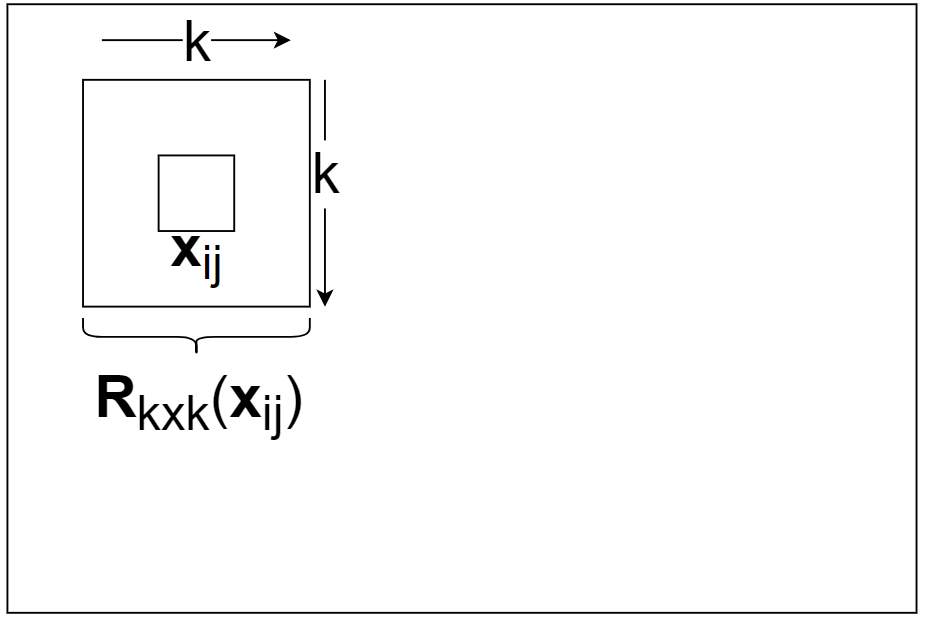
\includegraphics[scale=0.45]{images/LRX.PNG}
  \caption{ Visualization of a kernel of size $K$ $\times$ $K$ used in LRX. } 
  \label{fig:LRX}
\end{figure}


\subsection{Adaptive Causal Anomaly Detection}
\label{sec:ACAD_theory}
A variant of the RX AD is the Adaptive Causal Anomaly Detection (ACAD) \cite{chang2006characterization}. One issue of the RX algorithm is that previously detected anomalies with strong spectral signatures may have an impact upon the detection of later anomalies, as they may influence what is consider the background, which is shown in \cite{chang2006characterization}. ACAD is adaptive in the way that it builds a map of detected anomalies, and removes the previously detected anomaly pixel vectors from the causal sample correlation set. \\
Another benefit of ACAD relative to RX and LRX is that it may be computed in real-time. This is achieved by using the causal correlation matrix $\textbf{R}$($\textbf{x}_k$), defined in equation \ref{eq:caus_corr}, instead of the covariance or the correlation matrix computed on the global or a local set of pixel vectors, as in RX and LRX, respectively. In equation \ref{eq:caus_corr} $\textbf{x}_k$ is the observation test pixel vector, and $k$ is the index of the pixel vector currently being processed. The sum in equation \ref{eq:caus_corr} sums the correlation matrix for the pixel sample vectors {$\textbf{x}_1$, ....$\textbf{x}_k$}.  

\begin{equation}
    \textbf{R}(\textbf{x}_k)=\frac{1}{k}\sum_{i=1}^k\textbf{x}_i\textbf{x}_i^T. 
    \label{eq:caus_corr}
\end{equation}

To remove the previously detected anomalous pixel vectors from the correlation set, the sample spectral correlation matrix, referred to as the causal anomaly-removed sample spectral correlation matrix, is presented in equation \ref{eq:caus_corr_anomaly_removed}  \cite{chang2006characterization}:

\begin{equation}
    \Tilde{\textbf{R}}(\textbf{x}_k)= \textbf{R}(\textbf{x}_k) - \sum_{t_j\in\Delta(k)}\textbf{t}_j\textbf{t}_j^T ,
    \label{eq:caus_corr_anomaly_removed}
\end{equation}

where $\Delta(k)$ is the set of all earlier detected anomalous pixel vectors $\textbf{t}_j$ prior to the image pixel currently being processed, $\textbf{x}_k$.
\\
ACAD can then be defined as in equation \ref{eq:ACAD}:
\begin{equation}
    \delta^{ACAD}(\textbf{x}_k)= \textbf{x}_k^T\Tilde{\textbf{R}}^{-1}(\textbf{x}_k)\textbf{x}_k.
    \label{eq:ACAD}
\end{equation}

ACAD is a causal filter, meaning that only the pixels previously processed are used for anomaly detection.  It computes the correlation matrix for the previously captured pixel sample vector {$\textbf{x}_1$, ....$\textbf{x}_k$} up to the pixel currently being processed, $k$, as shown in equation \ref{eq:caus_corr}. This means that ACAD might be implemented in real-time and near-real time, as pixels can be processed as soon as they are captured by the push-broom HSI and the AD does not need to wait for the entire image to be loaded into memory. \\

An anomalous pixel vector have a significant spectral vector difference from its surroundings. Since ACAD is causal, the surroundings is defined as the $n_{acad}$ previously processed pixels. %To evaluate if a spectral vector is anomalous,
ACAD defines the variable $u_k$, used to evaluate if a pixel vector is anomalous, as shown in  equation \ref{eq:u_k}: 

\begin{equation}
    u_k = \frac{1}{n_{acad}}\sum_{i-1}^{n_{ACAD}}  \delta^{ACAD}(\textbf{x}_{k-i}).
    \label{eq:u_k}
\end{equation}

 In order to classify if a pixel vector is anomalous the variable $t_k$ is introduced, defined in equation \ref{eq:t_k}:
\begin{equation}
    t_k = \delta^{ACAD}(\textbf{x}_{k}) - u_k.
    \label{eq:t_k}
\end{equation}

 If $t_k$ is greater than a predetermined value $\tau$, the pixel vector is considered an anomaly an added to the set of anomalous targets. If not, it is used in subsequent data processing. 
The anomaly map created by ACAD is shown in equation \ref{eq:anomaly_map_ACAD}:
    
%\[
%    f(x)= 
%\begin{cases}
%    \frac{x^2-x}{x},& \text{if } x\geq 1\\
%    0,              & \text{otherwise}
%\end{cases}
%\]

\begin{equation}
    map_{ACAD}(\textbf{x}_{k}) =
   \left\{
   \begin{aligned}
    \Th 1\text{, if } t_k> \tau \\%(\flow_1)
    % &=  G \\
     \Th 0\text{, otherwise.}%(\flow_2) &= \ldots
   \end{aligned}
   \right.
   \label{eq:anomaly_map_ACAD}
\end{equation}



The four issues labelled Q1, Q2, Q3 and Q4 still remains. For a pixel vector to be considered anomaly it has to be relatively small compared to the size of the image. The relationship between the size of an anomaly and the size of the entire image is $\beta$, shown in equation \ref{eq:beta}:

\begin{equation}
    \beta  = \frac{Image\_size}{size\_of\_anomaly}.
    \label{eq:beta}
\end{equation}

According to \cite{chang2006characterization} empirical results show that $\beta$ will be $\approx$ 100.
The relationship between $\beta$ and $n_{ACAD}$ is shown in equation \ref{eq:n_acad}:
\begin{equation}
    n_{ACAD} = \frac{N}{\beta},
    \label{eq:n_acad}
\end{equation}

where $N$ is the total number of pixels in the image. In  RX and LRX, an earlier detected anomaly with a strong spectral signature may influence the detection of subsequent anomalies, as the anomalies are used for calculation of the correlation or covariance matrix. This is shown in Figure 12 in \cite{chang2006characterization}, where an anomaly with a strong spectral signature influences the RX detector in such a degree that it fails to detect four subsequent anomalous pixels. This problem is solved in ACAD by removing previously detected anomalous pixels from the sample spectral correlation matrix, as shown in equation \ref{eq:caus_corr_anomaly_removed}. 
\\


In \cite{chang2006characterization} noise-immunity tests have been done on different ADs, including RX and ACAD. These tests adds Gaussian noise with a Signal-to-noise ratio of 20:1, 10:1 and 5:1 to a test image. One of the conclusion is that the noise has less effects on ACAD compared to the RX detector as shown in Figure 13 in \cite{chang2006characterization}.
\\

%Might also be possible to do some binning?
%Benefits ACAD: \\
%- ACAD builds and updates an anomaly library and generates an anomaly map to provide spatial coordinates of all its detected anomalies in the original image. This anomaly map can also be used to classify all the detected anomalies. \\
%- ACAD can be considered to be real time, even though the data processing may take time. Once the processing of data is completed, the whole process of anomaly dettection is also completed at nearly the same time. 
%\\
%This implies that the performance of ACAD is not determined by the relative size of the entire image to the anomaly, but rather by the number of data sample vectors considered in $n_{acad}$.

%\\ Question
%\\ Causality; in causality, will the first pixel-vector processed have a high probability of being detected as a anomality?\\
%-Yes, might be an issue. Remedied by the ACAD according to the book.

%Note to self; include comparison here of the different Anomalies Detector


\subsection{Adaptive Local RX}
\label{sec:Adaptive_LRX_theory}
A modification of the LRX algorithm presented in section \ref{sec:LRX_theory} is the Adaptive Local RX (ALRX). This AD is a modification of LRX presented by the author. It is not yet described in literature (as far as the author knows). 
\\

ALRX is inspired by the anomaly-map creation and the removal of previously detected anomaly pixel vectors from the causal sample correlation set as done in the ACAD AD. Similarly, ALRX builds a anomaly map and removes previously detected anomaly pixel vectors that are located within the local window from the local sample correlation set. The result of the ALRX AD is shown in equation \ref{eq:ALRX}: 

\begin{equation}
    \delta_k^{ALRX}(\textbf{x}) = \textbf{x}^T\Tilde{\textbf{R}}_{k x k}(\textbf{x})^{-1}\textbf{x}.
    \label{eq:ALRX}
\end{equation}


\begin{equation}
   \Tilde{\textbf{R}}_{k x k}(\textbf{x})= \textbf{R}_{k x k}(\textbf{x})-\sum_{t_j\in\Delta(k_{KxK})}\textbf{t}_j\textbf{t}_j^T,
    \label{eq:ALRX_anomaly_removed}
\end{equation}

where $\Delta(k_{KxK})$ is the set of previously detected anomalous pixel vectors $\textbf{t}_j$ located within the local window of size $KxK$ with center in the image pixel vector currently being processed, $\textbf{x}$.

% INCLUDE the anomaly map creation and stuff

\section{Inverse matrix}
The computation of the inverse of a matrix is a part of all the considered ADs. This is a computationally intensive task. There exists multiple algorithms for computing the matrix inverse. One option is to do QR factorization \cite{QRD_fpga}, and compute the inverse of QR. In HW the QR-factorization is most often computed using Givens rotation enabled by a trigonometric algorithm called COrdinate Rotation DIgital Computer (CORDIC) \cite{CORDIC}. \\

Another option is to implement the inverse function by doing Gauss-Jordan elimination \cite{gauss_jordan_fpga}. The Gauss-Jordan elimination is highly parallelizable \cite{gauss_jordan_fpga}. A pseudo-code for computing the Gauss-Jordan elimination is shown in Figure \ref{fig:gauss_jordan_pseudocode}. The Gauss-Jordan elimination can be tiled into three parts; forward elimination, backward elimination and last division, marked by black, red and green square in Figure \ref{fig:gauss_jordan_pseudocode}. 
\begin{figure}[H]
\centering
   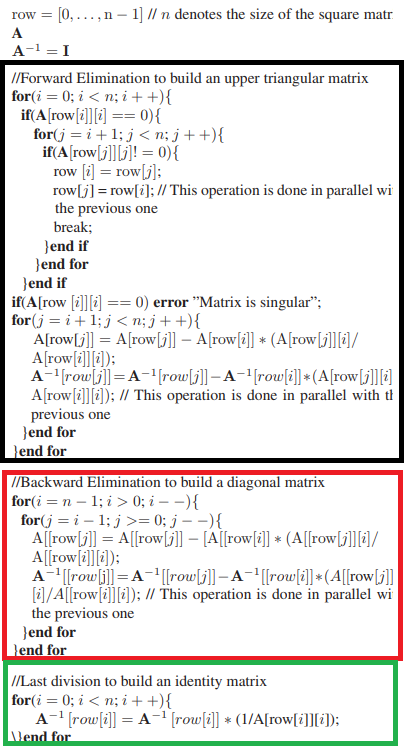
\includegraphics[scale=0.7]{images/gauss_jordan_pseudocode.png}
  \caption{ Pseudo-code for computing the inverse of a matrix by Gauss-Jordan elimination \cite{gauss_jordan_fpga}. } 
  \label{fig:gauss_jordan_pseudocode}
\end{figure}



\subsection{Gauss-Jordan elimination}
\label{sec:gauss_jordan_theory}
There are three different types of row operations performed on the rows of a matrix in Gauss-Jordan elimination:
\begin{enumerate}
\item Swap the positions of two rows. 
\item Multiply a row by a nonzero scalar. 
\item Adding a scalar multiple of one row to another.
\end{enumerate}  

\subsubsection{Forward elimination}
The first part of Gauss-Jordan elimination reduces the matrix to row echelon form (upper triangular matrix) by using row operations, starting at the topper-most row of the matrix, which is denoted as index zero, and iterating downwards. Two indexes are used, the outer index $i$ and the inner index $j$. This is shown in Figure \ref{fig:forward_elimination_pseudocode}. Forward elimination may use all of the different row operations listed, depending upon the existence of a zero element in the diagonal of the matrix.   

\begin{figure}[H]
\centering
   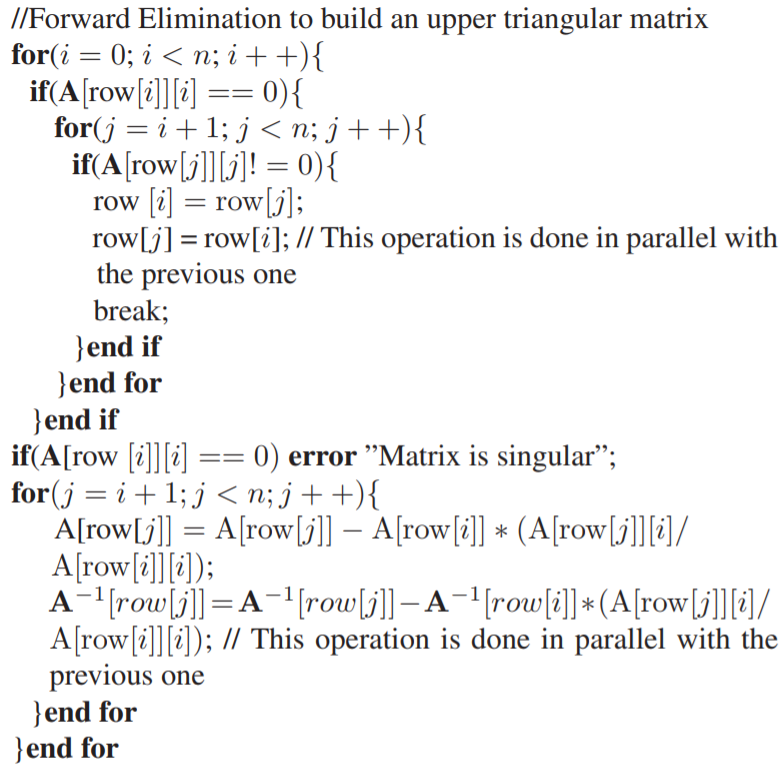
\includegraphics[scale=0.5]{images/forward_elimination_pseudocode.PNG}
  \caption{ Pseudo-code for computing the forward elimination in Gauss-Jordan elimination \cite{gauss_jordan_fpga}. } 
  \label{fig:forward_elimination_pseudocode}
\end{figure}


\subsubsection{Backward elimination}
Backward elimination utilizes row operation two and three in order to create a diagonal matrix. It starts at the bottom of the matrix, denoted index $P\_bands-1$ and iterates upwards. Two indexes are used, the outer index $i$ and the inner index $j$. This is shown in Figure \ref{fig:backward_elimination_pseudocode}.

\begin{figure}[H]
\centering
   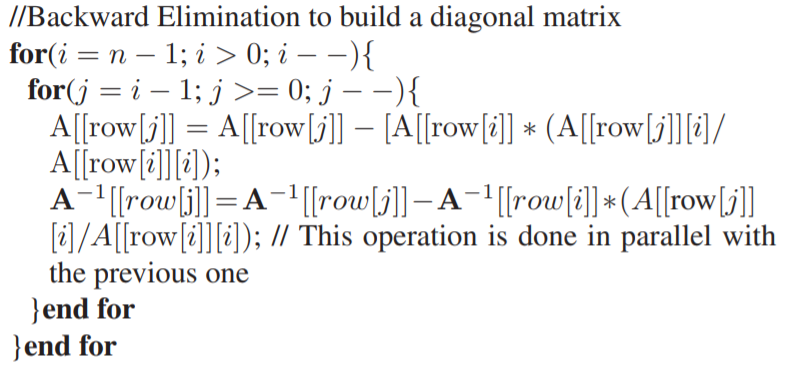
\includegraphics[scale=0.5]{images/backward_elimination_pseudocode.png}
  \caption{ Pseudo-code for computing the backward elimination in Gauss-Jordan elimination \cite{gauss_jordan_fpga}. } 
  \label{fig:backward_elimination_pseudocode}
\end{figure}


\subsubsection{Last division}
Last division is the last step of the Gauss-Jordan elimination. The last division starts at the topper-most index of the matrix and iterates downwards, shown in Figure \ref{fig:last_division_pseudocode}. It creates the matrix $A^{-1}$ by utilizing the second type of row operations. $A^{-1}$ is the inverse matrix of $A$; $A$ $\times$ $A^{-1}$ = $I$. $I$ is the identity matrix of size $P\_bands$ $\times$ $P\_bands$ containing zero elements, except for the diagonal of the matrix, which contains ones. 
\begin{figure}[H]
\centering
   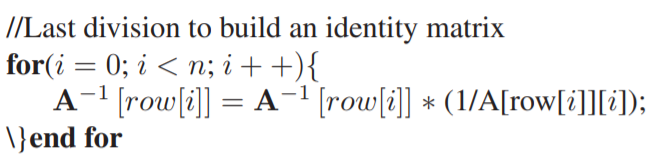
\includegraphics[scale=0.5]{images/last_division_pseudocode.png}
  \caption{ Pseudo-code for computing the last division in Gauss-Jordan elimination \cite{gauss_jordan_fpga}. } 
  \label{fig:last_division_pseudocode}
\end{figure}
%The Gauss-Jordan elimination is simpler to implement in HW than the method of QR-factorization method

%\subsection{QR-Factor}

%A QR-decomposition can certainly be used for matrix inversion because if A=QR then A−1=R−1Q−1=R−1QT and R−1 is easy to compute because R is triangular.\\
%Q-factor
%• Q is m × n with orthonormal columns (QTQ = I)
%• if A is square (m = n), then Q is orthogonal (Q^TQ = QQ^T = I)
%R-factor
%• R is n × n, upper triangular, with nonzero diagonal elements
%• R is nonsingular (diagonal elements are nonzero)

%\subsubsection{Givens rotation}

%Givens rotation can create an upper triangular matrix

